\documentclass[12pt,a4paper,oneside]{ctexart}
\usepackage{caption,graphicx,amsmath,amsthm,amsfonts,amssymb,bm,mathrsfs,extarrows,
indentfirst,setspace,textcomp,xcolor,color,colortbl,booktabs,float,subcaption,
fancyhdr,lipsum,tabularx,multirow,enumerate}
\usepackage[centering]{geometry}
\usepackage{array,blkarray}
\usepackage{tikz,tikz-3dplot,asymptote}
\usepackage{listings}

\geometry{left=2.5cm,right=2.5cm,top=2.5cm,bottom=2.5cm}
\usetikzlibrary{arrows.meta}
\setlength{\headheight}{15pt}
\newfontfamily\consolas{Consolas}
\definecolor{lightgray}{gray}{0.5}
\pagestyle{empty}
\setstretch{1.5}
\newcolumntype{C}{>{\centering\arraybackslash}X}

\newcommand{\dif}{\mathrm{d}}
\newcommand{\differ}{\backslash}
\newcommand{\ptl}{\partial}
\newcommand{\R}{\mathbb{R}}
\newcommand{\N}{\mathbb{N}}
\newcommand{\C}{\mathbb{C}}
\newcommand{\D}{\mathbb{D}}
\newcommand{\Z}{\mathbb{Z}}
\renewcommand{\phi}{\varphi}
\renewcommand{\epsilon}{\varepsilon}
\newcommand{\abs}[1]{\left\vert#1\right\vert}
\newcommand{\norm}[1]{\left\Vert#1\right\Vert}

\begin{document}
    \subsection*{第四问方差分析}
    黑:1,蓝绿:2,绿:3,浅蓝:4,浅绿:5,深蓝:6,深绿:7,紫:8。

    A:1,B:2,C:3。

    \begin{enumerate}[(1)]
        \item 方差分析纹饰.sav
        \item 方差分析颜色.sav
        \item 方差分析纹饰-输出.spv
        \item 方差分析颜色-输出.spv
    \end{enumerate}

    黑色:$\mathrm{CuO}$(刘仁玉),蓝绿色:$\mathrm{CuO},\mathrm{Fe_2O_3}$(李淑静,张瑜),绿色:$\mathrm{CuO}$(李宗志), 深蓝色:$\mathrm{Cu}^{2+}$
    (张瑜),浅蓝色:$\mathrm{Fe_2O_3},\mathrm{CuO},\mathrm{CaO}$(张瑜),浅绿:$\mathrm{Fe_2O_3}$ 深绿:$\mathrm{Fe_2O_3}$ 紫:$\mathrm{Na_2O},\mathrm{K_2O}$。
\end{document}


% !Mode:: "TeX:UTF-8"
% !TEX program  = xelatex

\documentclass[withoutpreface,bwprint]{cumcmthesis}
%\documentclass[withoutpreface,bwprint]{cumcmthesis} %去掉封面与编号页,电子版提交的时候使用。

\usepackage{setspace,multirow,tabularx,supertabular}
\setstretch{1.07}
\newcolumntype{C}{>{\centering\arraybackslash}X}

\usepackage{algorithm,algorithmicx,algpseudocode}
\renewcommand{\algorithmicrequire}{\textbf{Input:}}
\renewcommand{\algorithmicensure}{\textbf{Output:}}

\newcommand{\dif}{\mathrm{d}}
\newcommand{\differ}{\backslash}
\newcommand{\ptl}{\partial}
\newcommand{\R}{\mathbb{R}}
\newcommand{\N}{\mathbb{N}}
\newcommand{\C}{\mathbb{C}}
\newcommand{\D}{\mathbb{D}}
\newcommand{\Z}{\mathbb{Z}}
\renewcommand{\phi}{\varphi}
\renewcommand{\epsilon}{\varepsilon}
\newcommand{\abs}[1]{\left\vert#1\right\vert}
\newcommand{\norm}[1]{\left\Vert#1\right\Vert}
\newcommand{\mr}[1]{\mathrm{#1}}

\usepackage[framemethod=TikZ]{mdframed}
\usepackage{url}   % 网页链接
\usepackage{subcaption} % 子标题
\usepackage{rotfloat,makecell}
\usepackage{framed}
\usepackage{gbt7714}
\title{基于SVM支撑向量分类机与KMeans 聚类分析的古代玻璃成分分析模型}
\tihao{A}
\baominghao{4321}
\schoolname{XX大学}
\membera{ }
\memberb{ }
\memberc{ }
\supervisor{ }
\yearinput{2020}
\monthinput{08}
\dayinput{22}

\begin{document}
	
	\maketitle
	\begin{abstract}
	   
		
		针对玻璃文物的成分分析问题,本文建立了SVM 支撑向量机模型、KMeans 聚类分析模型,运用了卡方分析、独立样本t检验、包络线拟合、单因素方差分析等判断方法,提出了类型及亚类划分方案,并对多重指标与不同化学成分含量间的关系进行具体分析。
		
		针对问题一,为分析风化程度与基本信息间的关系,本文使用卡方分析法。首先根据成分比例累加和的约束筛选并对数据归一化处理;之后对指标组合进行卡方分析,得到玻璃风化程度与玻璃类型之间的渐进显著性为0.049,可以认为其具显著相关性,而风化程度与玻璃纹饰、颜色间并无显著相关性;最后结合统计柱状图得到可能与玻璃表面风化相关的组合,如(高钾,B,蓝绿)。
		
		为分类分析玻璃风化程度与化学成分含量的关系,本文采用相关性检验和独立样本t检验方法。首先按分类样本绘制雷达图得到直观的成分含量;之后通过计算Pearson相关系数判断每类样本中不同化学成分含量之间的相关性如高钾风化样品中CaO与$\mr{SiO_2}$,$\mr{Al_2O_3}$含量具有强负相关性;最后运用SPSS进行独立样本t检验,得到每种成分风化前后含量差异,如高钾玻璃风化前后$\mr{SiO_2}$、$\mr{K_2O}$、CaO、MgO、$\mr{Al_2O_3}$、$\mr{Fe_2O_3}$含量差异显著。
		                                          
		 为根据风化点检测数据预测未风化时各成分含量,根据独立样本t检验结果将化学成分分类,分别绘制风化前后差异明显的指标随$\mr{SiO_2}$含量变动的样本点,运用包络线拟合样本集中分布区域边界,代入风化前$\mr{SiO_2}$含量预测值实现多种成分的预测。      
		 
		 针对问题二,为分析玻璃类型及亚类分类规律,本文建立SVM支撑向量分类机模型与KMeans聚类分析模型 。首先通过求解二次规划问题,确定可将高钾、铅钡玻璃完全划分的最优超平面具体参数;其次通过绘制“$SSE$-聚类个数曲线” 找到合适的聚类个数,代入具体数据分别对高钾、铅钡玻璃实现聚类划分,得到铅钡玻璃的5个亚类)与高钾玻璃的3个亚类$D_i$ $(i=1,2,3)$;最后引入了豪斯多夫距离,克服了传统模型敏感性检验方法难以衡量集合偏移量的缺陷,验证了模型的稳健。
		 
		 针对问题三,为确定未分类文物所属类型及亚类,本文将文物数据依次代入问题二中求解的SVM支撑向量分类机模型与KMeans聚类分析模型,得到具体分类结果为A1、A6、A7属于高钾玻璃,A2、A3、A4、A5、A8属于铅钡玻璃,A1属于D2,A6、A7属于D0,A4、A8属于C4,A5属于C1。再对样本数据加入不同程度的Gauss噪声,依次代入两种模型,通过模型结果的准确性验证模型稳健性。
		 
		 针对问题四,为分析不同类别玻璃样品间化学成分含量的关联与差异,本文建立单因素方差分析模型。对于玻璃的类型、颜色、纹饰类别,首先结合问题二中求解的高钾铅钡玻璃分类规律,可得类型类别的分析结果;其次对其他两类分别进行方差分析,根据显著性大小得到不同颜色玻璃文物间含量差异较大的化学成分为CuO、PbO、SrO等,进而推测这些成分含量会是不同玻璃颜色的成因,而不同纹饰玻璃文物间化学成分含量无明显差异。
		 
		 综上,本文由数据驱动,运用SVM 支撑向量机  、KMeans聚类分析等多种模型方法实现了古代玻璃的成分分析,对于古代玻璃文物鉴别分类具有良好的适用性。
		 
		\textbf{关键词:卡方分析 独立样本t检验 SVM 支撑向量机  KMeans 聚类分析 单因素方差分析}
	\end{abstract}
	
	\section{问题背景与重述}
	\subsection{问题背景}
	玻璃通过丝绸之路从西方传入我国,成为了早期贸易往来的宝贵物证。研究表明,中国最晚自战国晚期便已经开发出了独特的玻璃配方{1},因此中国古代自制玻璃也具有与外来玻璃不同的化学成分。由于炼制过程中加入的助熔剂种类不同,玻璃成品中的主要化学成分往往也具有明显差异,继而我们可以把古代玻璃分为铅钡玻璃、钾钙玻璃、钠钙玻璃三类{3}。古代玻璃极易风化,这一过程中内外部元素大量交换往往导致其成分比例变化。研究风化导致的玻璃文物氧化物含量变动,不仅有助于考古工作者更准确地鉴别文物,也能对更好地保护玻璃文物带来启发。
	
	\subsection{问题重述}
	请根据所给的玻璃文物基本信息及化学成分比例数据建立模型,解决以下问题:
	
	问题 1:根据附件表单1的相关信息分析玻璃文物的表面风化与其玻璃类型、纹饰和颜色的关系;
	按照玻璃类型、文物样品表面有无风化分类,研究每一类中化学成分含量的统计规律。
	并根据风化点检测数据,预测其风化前的化学成分含量。
	
	问题 2:依据附件表单2数据分析高钾玻璃、铅钡玻璃的分类规律;
	对于每个类别选择合适的化学成分进行亚类划分,给出具体的划分方法及划分结果。
	再对分类结果的合理性和敏感性进行分析。
	
	问题 3:对附件表单3中未分类玻璃文物的化学成分进行分析,鉴别其所属类型,并对分类结果的敏感性进行分析。
	
	问题 4:针对不同类别的玻璃文物样品,分析其化学成分之间的关联关系,并比较不同类别之间的化学成分关联关系的差异性。
	\section{问题分析}
	\subsection{问题一的分析}
	在解决问题之前将进行数据的预处理,根据题中“将成分比例累加和介于
	85\%到105\%
	之间的数据视为有效数据”条件,初步筛选去掉范围外的数据,再将表中的数值归一化,保证每件文物各种成分占比和为1。
	
	针对问题一第一部分,为确定玻璃文物表面风化与基本信息间的关系,考虑到基本信息无偏序关系难以量化考量,拟采用定类变量法中的卡方分析。
	由于卡方分析具有“仅能分析两组指标间相关性”的局限性,未考虑三项基本信息的组合与玻璃风化程度间的相关性,因而将分别绘制风化玻璃类型、纹饰、颜色与未风化玻璃对应指标的统计图,
	进而综合考量玻璃风化程度与基本信息的两两关系和组合关系。
	
	针对问题一第二部分,为按类型分析风化前后各化学成分含量的统计规律,本文拟采用分类分析雷达图、相关性检验、独立样本t检验方法。
	首先为直观得到不同类型不同风化程度玻璃样品各成分含量,拟按分类样本分别绘制雷达图。通过观测雷达图,将得到每类样品化学元素含量的普遍规律。
	其次由于玻璃样品中化学元素种类丰富存在形式多样,猜测部分元素在风化过程中的变化具有线性关系。拟绘制散点图,若存在具有明显线性关系的元素组,则对其进行相关性检验,定量衡量相关性强弱。
	最后为了得到风化对高钾、铅钡玻璃内元素含量的影响,本文将分别对高钾、铅钡玻璃进行独立样本 t 检验,进而得到在不同显著性水平下呈现差异的化学成分。
	针对问题一第三部分,为根据风化后样本化学成分含量预测风化前对应含量,拟对铅钡玻璃、高钾玻璃样本点集中分布区域分别包络拟合预测。重点考虑此前独立样本t检验得出风化前后含量差异大的化学成分,求解这些成分随$\mr{SiO_2}$含量变化包络线,根据风化前$\mr{SiO_2}$含量的预测值,实现这些成分预测含量的求解。
	\subsection{问题二的分析:}
	针对问题二第一部分,为找出玻璃类型的分类规律,将玻璃样品看作化学成分指标空间上的点集,拟找出一种空间内的分割,使得高钾、铅钡玻璃能够被分割完全隔开,代入相关数据判断以超平面作为分割的合理性与可行性,若可行,求解得出具体模型结果。
	
	针对问题二第二部分,为对已按玻璃类型分类的样品进行亚类划分,使得亚类中样本性质相近,考虑采取 KMeans 聚类分析法,结合计算$SSE$随分簇数的变化趋势,确定合适的分簇数,对样本点进行聚类分析,可将位于同一聚类的元素归为同一亚类。
	
	针对问题二第三部分,为检验亚类划分模型的合理性与敏感性,考虑到样本数目有限,拟在传统方法上加以改进,将引入豪斯多夫距离作为衡量聚类偏移量的指标。当样本噪声大小保持在一定范围内时,若原聚类间豪斯多夫距离的最小值大于加入噪声后聚类偏移量之和,即可保证模型的稳健性。
	\subsection{问题三的分析:}
	针对问题三,为实现未分类样品的归类,拟将样品数据依次代入此前的SVM支撑向量机模型和 KMeans 聚类分析模型,找到样品所属玻璃类型与亚类。为实现分类结果的敏感性分析,对样品数据加入Gauss噪声,以与分类结果的相似度为正确率的评判标准,绘制“正确率——噪声大小”曲线,即可找到模型高正确率对应的噪声范围,继而在此范围内分类模型稳健。
	\subsection{问题四的分析:}
	针对问题四,为分析不同类别玻璃文物样品化学成分含量间的关联与差异,首先按玻璃类型、颜色、纹饰分类,拟对颜色、纹饰采用方差分析法,对玻璃类型采用问题三中的SVM支撑向量机模型。其次对不同类样品各项化学成分统计分析,最后还应结合相关文献,总结关联及差异。
	\section{模型假设}
	1)假设文物未检测出的化学成分近似为0。

	2)假设除了附件2中列出的化学成分之外,玻璃文物不包含其他的化学成分。

	3)假设不同玻璃文物化学成分含量之间没有关联。
	
	\section{符号说明}
	\begin{table}[H]
		\centering
		\
		\begin{tabularx}{\textwidth}{CC}
			\toprule
			符号 & 含义 \\
			\midrule
			$O_i$ & 第$i$类玻璃的观测频数\\
			$E_i$ & 第$i$类玻璃的期望频数\\
			$m_0$ & 每一类玻璃的样本数\\
			$\bm{a}=(a_1,\cdots,a_{14})$ & 每一类中的玻璃样本\\
			$a_j$ & 玻璃样本的各种化学成分含量\\
			$a_{jl}$ & 第$l$个样本的第$j$个化学成分含量\\
			$\bar{a}_j$ & 第$j$个化学成分含量的样本均值\\
			$\bm{a}_i$ & 每一类的第$i$个玻璃样本\\
			$D$ & 玻璃文物颜色种类\\
			$D_j$ & 玻璃文物的第$j$个颜色种类\\
			$n_j$ & 种类$D_j$下的数据量\\
			$E_{ij}$ & 第$i$个种类第$j$个文物化学成分含量\\
			\bottomrule
		\end{tabularx}
	\end{table}
	
	\section{问题一:}(***)
	可根据题意将问题一分为三个小问。第一小问通过卡方分析、绘制统计图表,找出玻璃文物表面风化与类型、纹饰、颜色之间的两两关系和组合关系。第二小问通过单因素方差分析,找出影响(高钾,风化)(高钾,未风化)(铅钡,风化)(铅钡,未风化)这四种类型玻璃文物的化学成分含量规律。第三小问通过聚类分析,将已分类玻璃文物划分为。。个聚类,可以认为同一聚类中的文物具有相似的风化化学成分条件,****,
	\subsection{问题一第一部分:分析玻璃文物表面风化与玻璃类型、纹饰、颜色间的关系}	
	为分析玻璃文物的表面风化与玻璃类型、纹饰、颜色间的关系,首先将风化程度与这三项基本指标分别组合,通过卡方分析得到对应的渐进显著性大小,进而与0.05比较说明组合内指标间的相关性。其次由于玻璃文物类型,纹饰,颜色之间存在一定的相关性,可以分别绘制在表面风化和表面未风化情况下其他各项指标样本的统计图。最后统计得到占比最高的指标组合与文物表面是否风化具有较强的相关性。
	
	\subsubsection{数据的预处理}
		首先根据题中“将成分比例累加和介于85\%到105\%之间的数据视为有效数据”这一信息,对附件表单2的数据进行清洗。不难发现15,17号玻璃文物成分比例累加分别为79.47\%、71.89\%不符合要求,故在数据集中删去其相关数据,在后续问题的解答中也不再使用相关信息。由于受到检测手段等限制,各成分比例累加和不一定为1,故不妨将所有成分占比归一化处理。
	\subsubsection{基于卡方分析的两两相关性判断}
   为分析风化情况与玻璃类型,风化情况与玻璃纹饰,风化情况与玻璃颜色之间的两两关系,考虑到基本信息间无偏序关系,不宜简单的赋值量化,故采用卡方分析的统计学原理求解其相关性。以风化情况与玻璃类型为例,此时可将风化、未风化与铅钡玻璃、高钾玻璃两两组合共得到4种分类情况$(m=4)$,将观测频数记为$O_i$$(i=1,2,\cdots,m)$。再假设这两项指标相互独立,可推出此时的期望频数$E_i$。
   
   那么Pearson卡方$\chi^2$为
   \begin{equation}
       \chi^2=\sum_{i=1}^m\frac{(O_i-E_i)^2}{E_i},
   \end{equation}
   
	代入附件表单1相关数据,计算可得:
	
	玻璃文物表面风化程度与的玻璃类型之间的渐进显著性为0.049$<$0.05,因此这两项指标之间具有显著相关性。
	
	玻璃文物表面风化程度与的玻璃纹饰之间的渐进显著性为0.057$>$0.05,这表明接受假设“这两项指标不相关”,同时拒绝备择假设“这两项指标显著相关”。
	
    玻璃文物表面风化程度与的玻璃颜色之间的渐进显著性为0.428$>$0.05,这表明这两项指标之间不具有显著相关性。
	
	
	\subsubsection{基于统计图的指标组合}
	其次考虑到玻璃类型、纹饰、颜色的不同组合对应的样本数目具有显著差异,例如符合(铅钡,A,浅蓝)组合有10种,而(铅钡,C,绿)仅有一组,故推测这三项指标之间具有一定的相关性。因而分别统计表面风化和未分化两种玻璃文物的相关信息,并绘制统计图如图\ref{fig:未风化分布图}、图\ref{fig:风化分布图}。
	
	\begin{figure}[H]
	\centering
	\subcaptionbox{未风化分布图\label{fig:未风化分布图}}{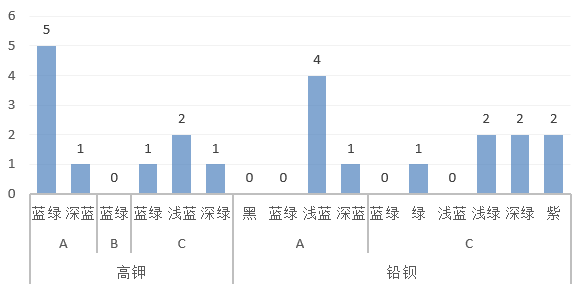
\includegraphics[scale=0.6]{未风化分布图.png}}
	\subcaptionbox{风化分布图\label{fig:风化分布图}}{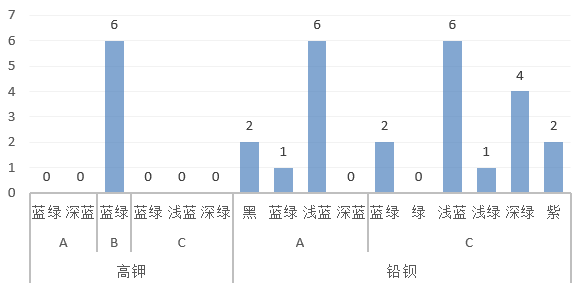
\includegraphics[scale=0.6]{风化分布图.png}}
	\caption{玻璃各特征的分布}
\end{figure}
	
	由图一知,在表面风化的玻璃文物中,高钾玻璃仅有(高钾,B,蓝绿)这一种,铅钡玻璃则多以(铅钡,A,浅蓝)(铅钡,C,浅蓝)(铅钡,C,深绿)的组合形式出现,可以推测玻璃文物表面风化与三项指标的上述四种组合相关。
	
	由图二知,在表面未风化的玻璃文物中,(高钾,A,蓝绿)(铅钡,A,浅蓝)是主要的组合形式,故可以推测玻璃文物表面未风化与这两种组合相关。

	\subsection{问题一第二部分:分类分析化学成分含量的统计规律}
	为按玻璃类型分析玻璃表面有无风化化学成分含量的统计规律,首先将样本分为高钾风化、高钾未风化、铅钡风化、铅钡未风化四种,分别绘制各成分含量占比雷达图,得到直观的统计规律。其次可以通过计算Person相关系数分别对高钾样本风化前后数据和铅钡样本风化前后数据进行相关性检验。最后可以再进行独立样本t检验,找出不同类型玻璃样本风化前后化学含量变化显著的成分。
	\subsubsection{各化学成分含量雷达图}
	为了直观表示样本各化学成分的含量,利用按玻璃类型、玻璃表面有无风化分类的4种样本数据分别绘制各化学成分含量雷达图如图:
	
\begin{figure}[H]
	\centering
	\subcaptionbox{高钾无风化玻璃各化学成分雷达图\label{fig:高钾无风化雷达}}{
	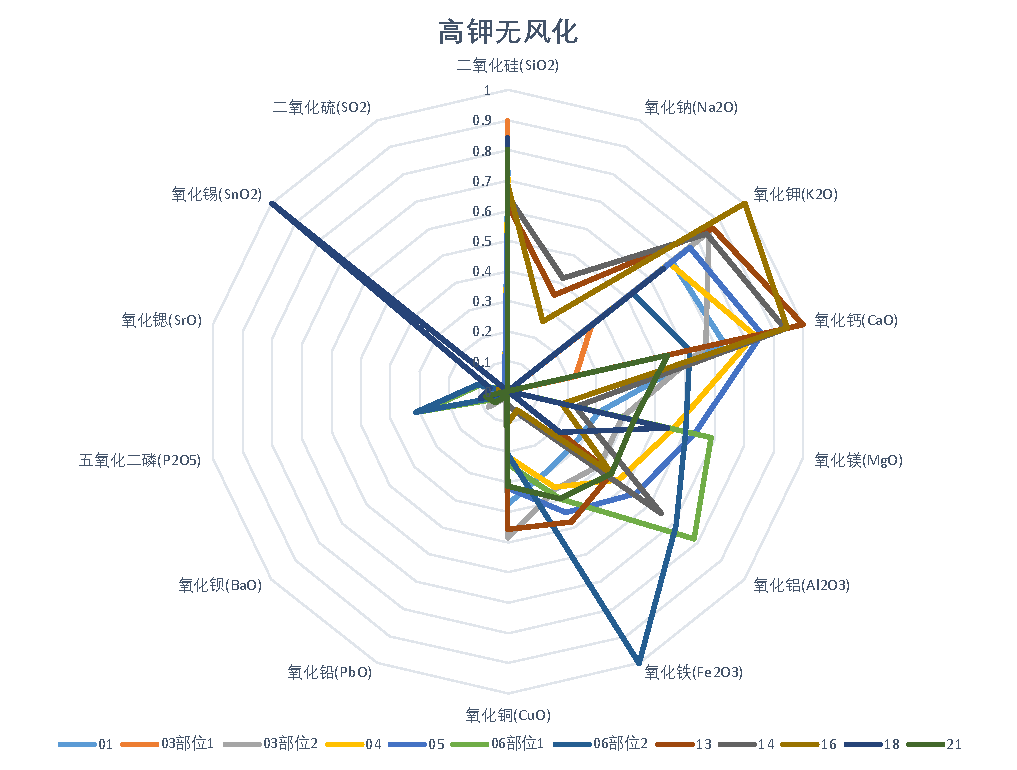
\includegraphics[scale=0.4]{高钾无风化.pdf}
	}
	\subcaptionbox{铅钡无风化玻璃各化学成分雷达图\label{fig:铅钡无风化雷达}}{
	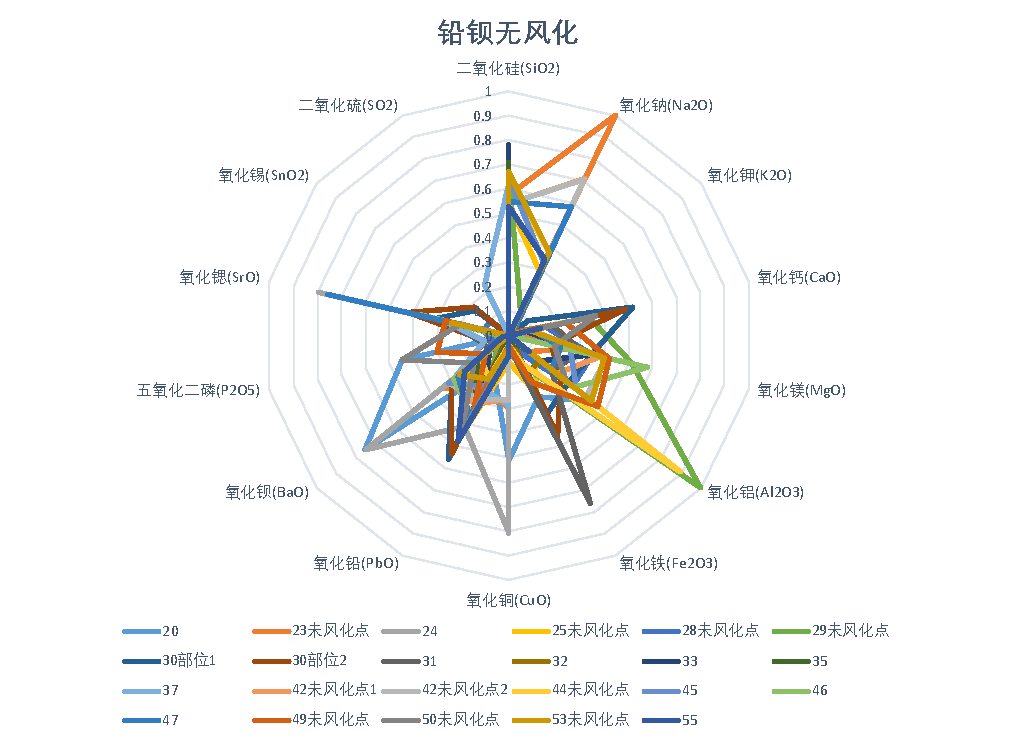
\includegraphics[scale=0.4]{铅钡无风化.pdf}
	}
	\subcaptionbox{高钾风化玻璃各化学成分雷达图\label{fig:高钾风化雷达}}{
	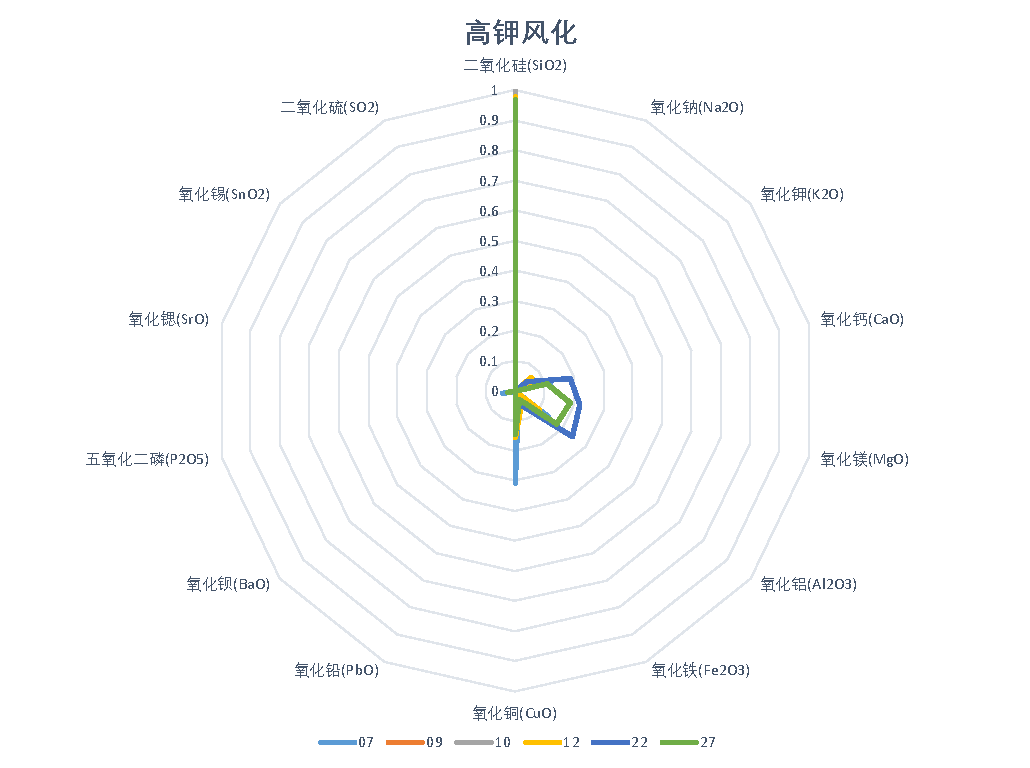
\includegraphics[scale=0.4]{高钾风化.pdf}}
	\subcaptionbox{铅钡风化玻璃各化学成分雷达图\label{fig:铅钡风化雷达}}{
	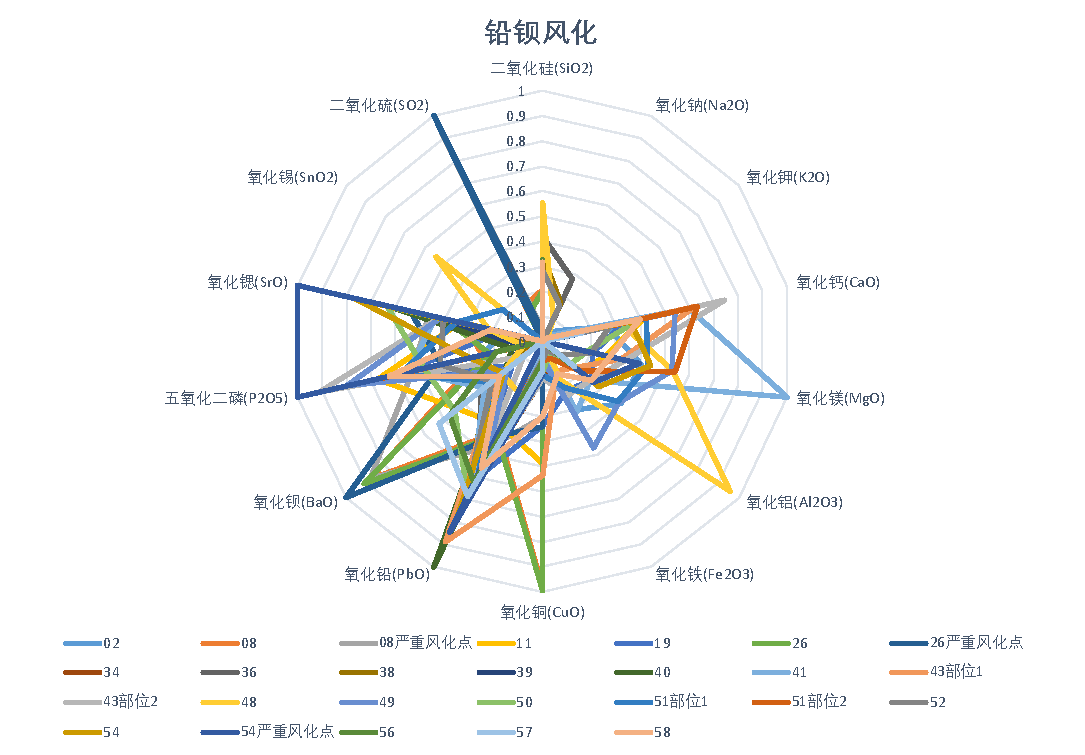
\includegraphics[scale=0.4]{铅钡风化.pdf}}
	\caption{风化玻璃}
	\label{fig:未风化雷达图}
\end{figure}

	在高钾风化样本中,样本$\mr{SiO_2}$含量占比普遍较高,$\mr{MgO}$,$\mr{CuO}$含量极低。
	
	在高钾未风化样本中,样本$\mr{CaO}$,$\mr{K_2O}$含量最高,$\mr{SiO_2}$,$\mr{Fe_2O_3}$,$\mr{Al_2O_3}$含量也相对较高。
	
	在铅钡无风化样本中,样本$\mr{PbO}$,$\mr{CaO}$,$\mr{Fe_2O_3}$含量较高,其余组分含量相差较大,但普遍具有少量$\mr{BaO}$。
	
	在铅钡风化样本中,样本$\mr{PbO}$,$\mr{BaO}$,$\mr{P_2O_5}$含量最高,$\mr{SrO}$,$\mr{CaO}$,$\mr{MgO}$含量相对较高。
	
	\subsubsection{相关性检验}
	\label{se:相关性检验}
	考虑到样本中$\mr{SiO_2}$占比较高,且在高钾玻璃风化过程中随着表面富硅层的形成$\mr{SiO_2}$含量逐渐上升、在铅钡玻璃风化过程中$\mr{SiO_2}$侵蚀流失严重含量逐渐下降\cite{刘松2011},由于各种元素占比和在进行归一化后均为一,故推测不同类型样品中部分氧化物与$\mr{SiO_2}$含量呈负相关性或正相关性。
	
	我们绘制部分氧化物随$\mr{SiO_2}$含量变化的散点图如图(***)
	
	观察发现,***等氧化物与$\mr{SiO_2}$含量呈明显的相关关系,故考虑
	用Pearson相关性检验分析高钾无风化、高钾风化、铅钡无风化、铅钡风化这四种样本中每种化学成分的具体相关性强弱。不妨以高钾无风化样本为例,用$\bm{a}=(a_1,a_2,\cdots,a_{14})$表示第$i$件高钾无风化玻璃文物,其中$a_j\ (j=1,\cdots,14)$按$j$递增依次为$\mr{SiO_2},\cdots,\mr{SO_2}$等化学成分指标。那么对于其中两个不同的成分$a_j,a_k\ (j\neq k)$,它们的Pearson相关系数为 
	\begin{equation}
	    r_{jk}=\frac{\sum_{l=1}^{m_0}(a_{jl}-\bar{a}_j)(a_{kl}-\bar{a}_k)}{\left(\sum_{l=1}^{m_0}(a_{jl}-\bar{a}_j)^2\right)^{1/2}\left(\sum_{l=1}^{m_0}(a_{kl}-\bar{a}_k)^2\right)^{1/2}},
	\end{equation}
    其中$a_{jl}$表示第l个样本的第j项化学成分,$\bar{a}_j$,$\bar{a}_k$是这些成分的样本均值。
    
    计算得到的Pearson相关系数可以表征两种成分的相关性,得到结果如图(***)。
    
    
    图(***)仅展示部分氧化物的显著性大小,完整图表见附录(***)。根据判别准则,当显著性小于0.05时,说明两种成分相关性较强;当显著性大于0.05,说明两种成分相关性不强。当相关性较强时,Pearson相关系数大于0,说明正相关性较强;小于0时,说明负相关性较强。
    
    观察可得:(这里只集中描述在0.01级别下极强的相关关系)
    
    在高钾风化玻璃样品中,CaO与$\mr{SiO_2}$,$\mr{Al_2O_3}$含量具有极强的负相关性。
    
    在铅钡无风化玻璃样品中,$\mr{SiO_2}$与PbO,BaO含量具有极强的负相关性,PbO、CaO与$\mr{SnO_2}$含量具有极强的正相关性,CuO与BaO含量具有极强的正相关性。
    
    在铅钡风化玻璃样品中,$\mr{SiO_2}$与$\mr{SrO}$,$\mr{SO_2}$含量具有极强的负相关性,$\mr{SiO_2}$与$\mr{Al_2O_3}$,$\mr{SnO_2}$含量具有极强的正相关性;CaO与MgO、$\mr{Fe_2O_3}$含量具有极强的正相关性,MgO与$\mr{Al_2O_3}$、$\mr{Fe_2O_3}$含量具有极强的正相关性;MgO与BaO有极强的负相关性;$\mr{Al_2O_3}$与$\mr{Fe_2O_3}$、$\mr{SnO_2}$含量具有极强的正相关性;BaO与$\mr{SO_2}$含量具有极强的正相关性。
    
	
	\subsubsection{独立样本t检验}
	\label{se:独立样本t检验}
	
	根据类型将玻璃文物样品分为高钾和铅钡两类,为针对每类玻璃分析文物风化前后化学成分含量这两组定量数据间的关系,考虑使用SPSS进行独立样本t检验。
	
	首先进行莱文方差等同性检验判断数据是否具有方差齐性,再根据结果分别进行平均值等同性t检验。得到铅钡、高钾类玻璃文物样品检验结果如图(***)

    根据检验标准,高钾玻璃风化前后$\mr{SiO_2}$、$\mr{K_2O}$、CaO、MgO、$\mr{Al_2O_3}$、$\mr{Fe_2O_3}$含量在 0.01 显著性水平下呈现明显差异,这说明了风化会对高钾玻璃中这些化学成分含量产生较大影响。
    
    铅钡玻璃风化前后$\mr{SiO_2}$、$\mr{Na_2O}$、CaO、PbO、$\mr{P_2O_5}$含量在 0.01 显著性水平下呈现明显差异,SrO含量在0.05 显著性水平下呈现明显差异,这说明了风化会对铅钡玻璃中这些化学成分含量产生较大影响。
    \subsection{问题一第三部分:预测风化点风化前化学成分含量}
    
    由于不同类型玻璃文物样本之间元素变化趋势存在较大差异,故考虑分别对高钾、铅钡玻璃进行风化前化学成分含量预测。
    
    以铅钡玻璃为例,通过\ref{se:独立样本t检验}中独立样本t检验,发现风化会对铅钡玻璃中$\mr{SiO_2}$、$\mr{Na_2O}$、CaO、PbO、$\mr{P_2O_5}$、SrO含量产生较大影响;对$\mr{K_2O}$、MgO、$\mr{Al_2O_3}$、$\mr{Fe_2O_3}$、CuO、BaO、$\mr{SnO_2}$的含量影响不大,因此可以忽略风化对这些化学成分含量造成的影响。对分化后含量基本为0的$\mr{Na_2O}$无法采用拟合预测,故取风化前平均值0.927212作为对其风化前含量的预测结果。
    对仅在严重风化情况下才会出现的$\mr{SO_2}$,预测其风化前含量为0。
    
    下面只需对玻璃文物风化前$\mr{SiO_2}$、CaO、PbO、$\mr{P_2O_5}$、SrO含量进行预测。在\ref{se:相关性检验}中的相关分析表明,可以用$\mr{SiO_2}$含量作自变量,绘制“其他元素——二氧化硅”的样本散点分布图,如图\ref{fig:高钾类玻璃包络线拟合}和\ref{fig:铅钡类玻璃包络线拟合}。
    
    \begin{figure}[H]
	\centering
	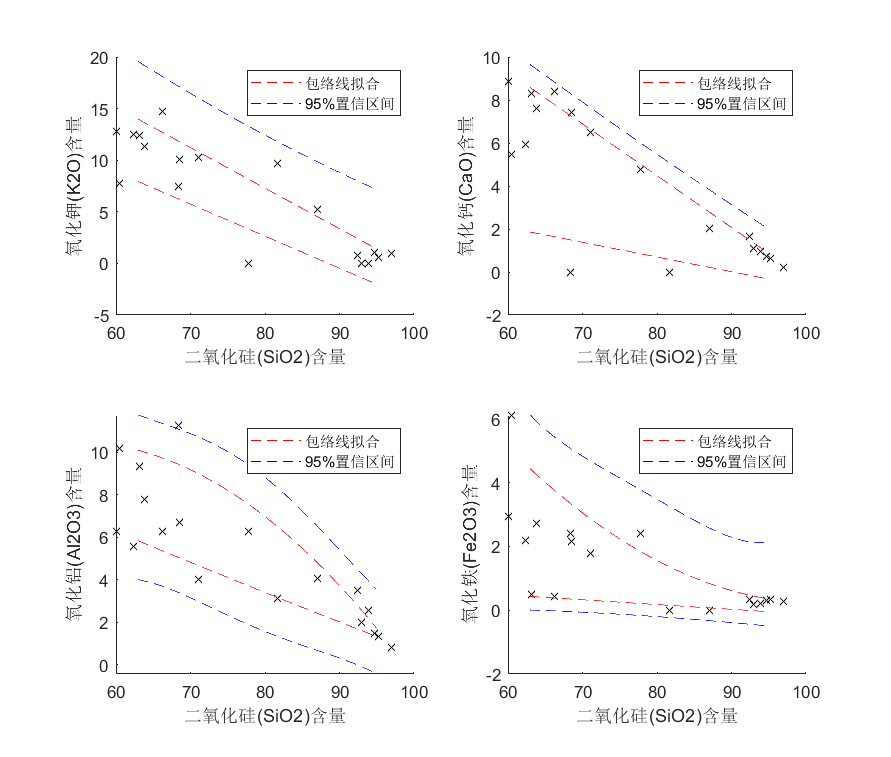
\includegraphics[scale=0.5]{高钾类玻璃包络线拟合.png}
	\caption{高钾类玻璃包络线拟合}
	\label{fig:高钾类玻璃包络线拟合}
\end{figure}

\begin{figure}[H]
	\centering
	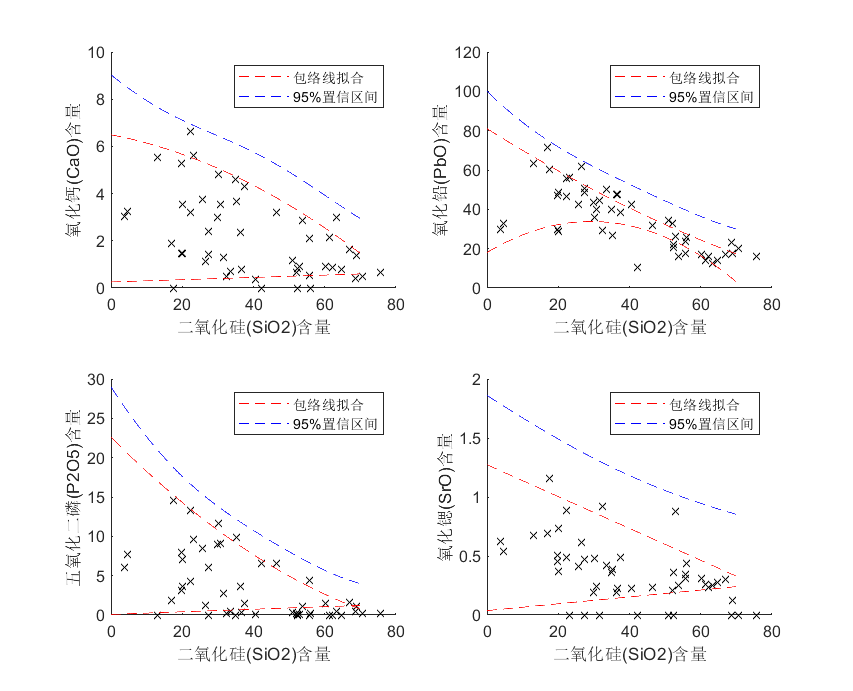
\includegraphics[scale=0.5]{铅钡类玻璃包络线拟合.png}
	\caption{铅钡类玻璃包络线拟合}
	\label{fig:铅钡类玻璃包络线拟合}
\end{figure}
	
	观察发现,样本点集中分布在图中的特定区域,但无明显函数规律,故考虑用两条包络线对分布区域的上下边界分别进行拟合。
	以CaO为例,将对分布边界拟合得到包络线表达式记为$f_i(x)$($f_i(x)=a_nx^n+a_{n-1}x^{n-1}+\cdots+a_1x+a_0$,当i=0时表示上界拟合函数,当i=1时表示下届拟合函数),针对风化后样本点$(x_0),y_0)$其中$x_0$表示$\mr{SiO_2}$含量,$y_0$表示$\mr{CaO}$含量。记$g(x)=f(x)+b$,求解$g(x_0)=y_0$得到b,就针对这一样本点求出了化学成分含量拟合曲线。
	
	得到结果如下:
	% Table generated by Excel2LaTeX from sheet 'Sheet2'
\begin{table}[H]
	\centering
	\caption{铅钡类玻璃文物}
	  \begin{tabular}{rlrr}
	  \toprule
	  \multicolumn{1}{r}{\multirow{2}[4]{*}{氧化钙}} & $f_0(x)=-0.00061x^2-0.02916x+6.493919$ &       &  \\
  \cmidrule{2-4}          & $f_1(x)=0.004909x+0.25342$ &       &  \\
	  \midrule
	  \multicolumn{1}{r}{\multirow{2}[4]{*}{氧化铅}} & $f_0(x)=0.003257x^2-1.13898x+81.04876$ &       &  \\
  \cmidrule{2-4}          & $f_1(X)=-0.01846x^2+1.079242+18.04178$ &       &  \\
	  \midrule
	  \multicolumn{1}{r}{\multirow{2}[4]{*}{五氧化二磷}} & $f_0(x)=0.002049x^2-0.45591x+22.62081$ &       &  \\
  \cmidrule{2-4}          & $f_1(x)=0.016274x+0.081324$ &       &  \\
	  \midrule
	  \multicolumn{1}{r}{\multirow{2}[4]{*}{氧化锶}} & $f_0(x)=-0.01349x+1.273419$ &       &  \\
  \cmidrule{2-4}          & $f_1(X)=0.002906x+0.037155$ &       &  \\
	  \bottomrule
	  \end{tabular}%
	\label{tab:铅钡类玻璃文物}%
  \end{table}%

% Table generated by Excel2LaTeX from sheet 'Sheet2'
\begin{table}[H]
	\centering
	\caption{铅钡类玻璃文物}
	  \begin{tabular}{rl}
	  \toprule
	  \multicolumn{1}{r}{\multirow{2}[4]{*}{氧化钙}} & $f_0(x)=-0.00061x^2-0.02916x+6.493919$\\
  \cmidrule{2-2}          & $f_1(x)=0.004909x+0.25342$\\
	  \midrule
	  \multicolumn{1}{r}{\multirow{2}[4]{*}{氧化铅}} & $f_0(x)=0.003257x^2-1.13898x+81.04876$\\
  \cmidrule{2-2}          & $f_1(X)=-0.01846x^2+1.079242+18.04178$\\
	  \midrule
	  \multicolumn{1}{r}{\multirow{2}[4]{*}{五氧化二磷}} & $f_0(x)=0.002049x^2-0.45591x+22.62081$ \\
  \cmidrule{2-2}          & $f_1(x)=0.016274x+0.081324$\\
	  \midrule
	  \multicolumn{1}{r}{\multirow{2}[4]{*}{氧化锶}} & $f_0(x)=-0.01349x+1.273419$\\
  \cmidrule{2-2}          & $f_1(X)=0.002906x+0.037155$\\
	  \bottomrule
	  \end{tabular}%
	\label{tab:铅钡类玻璃文物函数}%
  \end{table}%


	通过相关文献可知未风化铅钡玻璃文物中$\mr{SiO_2}$含量约为$47.96\%\sim72.61\%$,综合考量附件表单2中未风化铅钡玻璃$\mr{SiO_2}$数据,认为未风化铅钡玻璃含量为$50\%\sim70\%$,将风化后每个样本点数据依次代入拟合曲线,得出铅钡玻璃样品风化前CaO含量预测值的上下界,例如:预测**号样品风化前CaO含量上界为****,下界为
	
    同理,对已风化铅钡玻璃和高钾玻璃其他化学成分含量分别拟合,得到风化前各化学成分预测结果。(详见附录)
	
	\section{问题二:}
	由题意,问题二由三部分组成。第一部分为了找出高钾、铅钡玻璃的分类规律,采用SVM支撑向量分类机进行划分;第二部分为对每个类别的分类样品进行亚类划分,建立KMeans 聚类分析模型,将化学成分含量相近的样品归为同一聚类,构成亚类划分;第三部分中,为检验分类方式合理性与敏感性,在原有数据集的基础上加入随机分布的高斯噪声并重新进行分类,比较前后分类结果的差别以说明模型的合理性和稳定性,并最后证明了模型的稳健。
	\subsection{问题二第一部分:SVM分类机分析高钾、铅钡玻璃的分类规律}
        古代玻璃分为高钾、铅钡玻璃的分类方式,只和玻璃的化学组成成分相关,而与玻璃的颜色、纹饰无关。由于已有高钾、铅钡玻璃分类标签,对于该有标签的数据集,非常适合采用SVM支撑向量分类机,采用有监督的学习方式,以找出在玻璃的化学组成成分$\R^{14}$空间上,将玻璃划分为高钾和铅钡玻璃的分界超平面
    
	本文建立SVM支撑向量分类机模型如下。将铅钡玻璃、高钾玻璃的每种化学成分都看作一个维度,将这些样本点看作$\R^{14}$空间上的坐标,记为$\bm{a}_i$($i$=1,2$,\cdots,67$将同一文物的两个取样点对应的化学成分视作两个样本)。为找到$\R^{14}$空间上的超平面,将整个空间分成两部分,保证高钾玻璃和铅钡玻璃分别位于这两个不同的部分中。对高钾玻璃标签,以代号0表示;对铅钡玻璃标签,以代号1表示。

  由于数据量较少,为了避免过拟合现象的发生,将样本数据划分为训练集和测试集两个部分。用训练集训练SVM支撑向量分类机,测试集测试该分类器的表现。如果该分类器在测试集上表现良好,则能说明模型分类有效且未出现过拟合。

  首先随机抽取80\%的样本数据作为训练集,将目标划分的超平面记为
  $$H=\left\{ \bm{x}\in \mathbb{R}^{14}| (\bm{\omega} \cdot \bm{x})+b=0\right\}$$
  
  其中$\bm{\omega}$,$b$为参数。
  分类需要保证铅钡玻璃对应的训练样本点集$\omega_{1}$均在超平面上部, 高钾玻璃对应的训练样本点集$\omega_{2}$均在超平面下部,此外再保证超平面到两个点集的最近距离都尽可能地远,即最大化普通支持向量间的间隔$\frac{2}{\left\| \bm{\omega } \right\|}$,就有
  \begin{equation*}
      \begin{array}{ll}
          \max & \frac{2}{\|\bm{\omega}\|} \\
          \mathrm{s.t.} & \begin{cases}
          (\bm{\omega}\cdot\bm{a}_i)+b\geqslant y_i, & y_i=1,\quad i\in \omega_1\\
          (\bm{\omega}\cdot \bm{a}_i)+b\leqslant y_i,&y_i=-1,\quad i\in\omega_2\end{cases}
      \end{array}
  \end{equation*}
  那么寻找最优超平面的问题可转化为求解二次规划问题\cite{司守奎2015}。
  \begin{equation*}
      \begin{array}{ll}
          \min & \frac{1}{2}\|\bm{\omega}\|^2, \\
          \mathrm{s.t.} & y_i[(\bm{\omega}\cdot\bm{a}_i)+b]\geqslant 1,\quad i=1,\cdots,67
      \end{array}
  \end{equation*}
  
  为求解这一问题,
  引入Lagrange函数
  
  $$L(\bm{\omega,b,\bm{\alpha}})=\frac{1}{2}\Vert \bm{\omega}\Vert^2+\sum_{i=1}^l\alpha_i\{1-y_i[\bm{\omega}\cdot \bm{a}_i+b]\},$$
  
  式中: $ \boldsymbol{\alpha}=\left[\alpha_{1} \cdots, \alpha_{67}\right]^{\mathrm{T}}$为Lagrange乘子。
  原问题可转化为求解最优化问题(****)
  \begin{equation*}
    \begin{array}{ll}
        \max_{\bm{\alpha}} & -\frac{1}{2}\sum_{i=1}^{67}\sum_{j=1}^{67}y_iy_j\alpha_i\alpha_j(\bm{a}_i\cdot\bm{a}_j)+\sum_{i=1}^{67}\alpha_i, \\
        \mathrm{s.t.} & \begin{cases}
            \sum_{i=1}^{67}y_i\alpha_i=0\\
            \alpha_i\geqslant 0,i=1,\cdots,67
            \end{cases}
    \end{array}
\end{equation*}
  
  代入训练样本点数据,可得
  
  $\bm{\omega} =(-0.02956241,0.00551535,-0.05283312,-0.01644926,-0.00040758,0.03743216,\\-0.02505811,-0.01378527,0.10249466,0.01348478,-0.02241906,0.00158788,0,0)$
  
  $b=1.1452272$
  
  将剩下的20\%样本点数据代入超平面进行验证,得到准确为1.0,即所有的测试集数据均被正确的划分。这就说明了SVM支撑向量机方法的可行性,表明通过超平面,可以正确的依据$\R^{14}$空间上的玻璃化学组成成分,将其划分为高钾和铅钡玻璃。

    由前所述,高钾玻璃的标签表示为0,铅钡玻璃的标签表示为1,则对于一化学成分组成已知的点,将其化学组成成分${\bm{x}}$代入超平面方程${(\bm{\omega} \cdot \bm{x})+b}$:若该点位于超平面之上${((\bm{\omega} \cdot \bm{x})+b >0)}$,则为铅钡玻璃;反之若该点位于超平面之下${((\bm{\omega} \cdot \bm{x})+b<0)}$,则为高钾玻璃。因此,对于该表现有效的SVM支撑向量机,可以通过其超平面的参数方程${(\bm{\omega} \cdot \bm{x})+b=0}$(${\bm{\omega}}$,$b$ 如上所示),分析得到高钾玻璃、铅钡玻璃的分类规律。

    ${\bm{\omega}}$中绝对值较大的分量为${\bm{\omega}_3,\bm{\omega}_6,\bm{\omega}_9}$,对应的化学组分为氧化钾、氧化铝、氧化铅,其中${\bm{\omega}_3}$的值为负,说明样品含有的氧化钾较高时,倾向被分类为高钾玻璃;而${\bm{\omega}_6,\bm{\omega}_9}$的值为正,说明样品含有的氧化铝和氧化铅含量较高时,倾向于被分类为铅钡玻璃。
    
    ${\bm{\omega}}$中绝对值较小的分量为${\bm{\omega}_2,\bm{\omega}_5,\bm{\omega}_{12},\bm{\omega}_{13},\bm{\omega}_{14}}$,对应的化学组分为氧化钠、氧化镁、氧化锶、氧化锡、二氧化硫。说明样品中含有的该组分含量多少,对玻璃划分为高钾玻璃和铅钡玻璃的影响性较小。

    
	\subsection{问题二第二部分:选择合适化学成分,由KMeans聚类分析划分玻璃类别亚类}
	为了依据化学成分实现对高钾玻璃、铅钡玻璃的亚类划分,首先需要进行化学成分的合理选取。
	相关文献表明:高钾玻璃在风化过程中,碱金属元素组分变动显著,如Na,K元素流失严重,而随着风化表面形成富硅层,Si元素占比明显上升。铅钡玻璃在风化过程中,由于发生了水解氢化反应,Pb,Si含量明显增加,Ba含量显著降低。[刘松***]此外在实际选取指标时,为了得到层次清晰类别显著的聚类划分结果,还需要确保样本对应的指标方差大小适中,如果选取指标对应的方差太小,则说明在该类别中该指标的变动范围不大,不适应作为相关指标。
	
	综合考虑上述因素,我们以Si,K作为高钾玻璃的划分指标,以Pb,Ba,Si作为铅钡玻璃的划分指标。
	
    对于同一类型的玻璃,其亚类应有化学成分相近的特点,不同亚类之间化学组分应有明显差距。表现在由其各化学成分构成的$\R^{n}$空间上,存在点集集中分布的趋势。故采取KMeans聚类分析法来找出点集的亚类。

    为了找出最适合的聚类数目,采用各个点到聚类中心的距离平方和SSE来衡量
    \begin{equation*}
        SSE=\sum_{C_j}^m\sum_{\bm{x}_j^{(i)} \in C_j}||\bm{x}_j^{(i)} -\mu^{(j)}||_2^2
    \end{equation*}
    ${C_1,C_2,...,C_m}$为聚类结果,为各个聚类的点集
    
        
	首先绘制样本点簇内误差平方和($SSE$)与聚类个数的图像,如图
	(或者合并成一个图********)
\begin{figure}[H]
	\begin{subfigure}[t]{.515\linewidth}
	\centering
	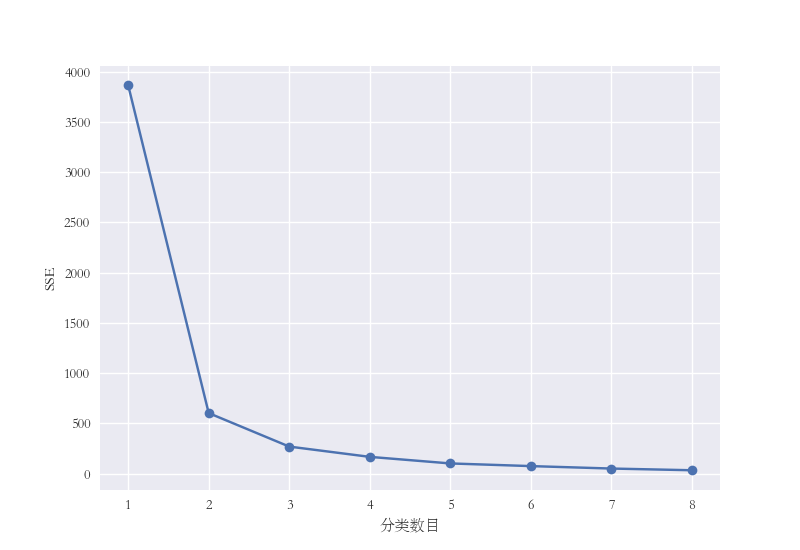
\includegraphics[width=.9\linewidth]{高钾类SSE.png}
	\caption{高钾类玻璃样本$SSE$}
	\label{fig:高钾类玻璃样本$SSE$}
	\end{subfigure}
	\begin{subfigure}[t]{.515\linewidth}
	\centering
	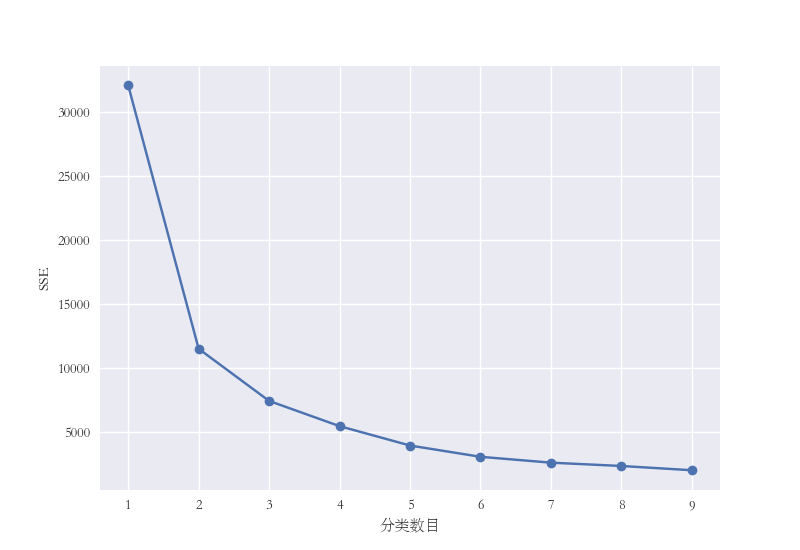
\includegraphics[width=.9\linewidth]{铅钡类SSE.png}
	\caption{铅钡类玻璃样本$SSE$}
	\label{铅钡类玻璃样本$SSE$}
	\end{subfigure}
	\caption{$SSE$与分类数目的关系}
	\end{figure}

	
	观察发现,SSE存在迅速下降过拐点后继而缓慢下降下降的变化趋势。在SSE迅速下降的时,说明各个点离其聚类中心的距离在迅速变小,模型的分类个数增加是有效的。在SSE下降缓慢时,说明此时增加分类数已经不能有效减小各个点离其聚类中心的距离,模型出现过拟合。故采取下降趋势的拐点作为应当分类的亚类个数。即铅钡玻璃样本分成5个聚类、高钾玻璃样本分成3个聚类。
	
	\begin{figure}[H]
	\centering
	\begin{subfigure}[t]{0.47\linewidth}
		\centering
		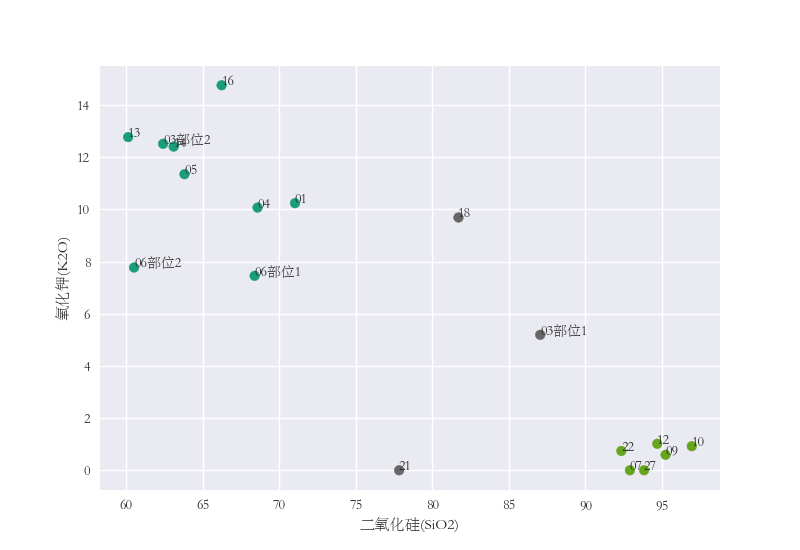
\includegraphics[width=0.9\linewidth]{高钾类玻璃聚类分析结果.png}
		\caption{高钾类玻璃聚类分析结果}
		\label{fig:高钾类玻璃聚类分析结果}
		\end{subfigure}
		\begin{subfigure}[t]{0.47\linewidth}
		\centering
		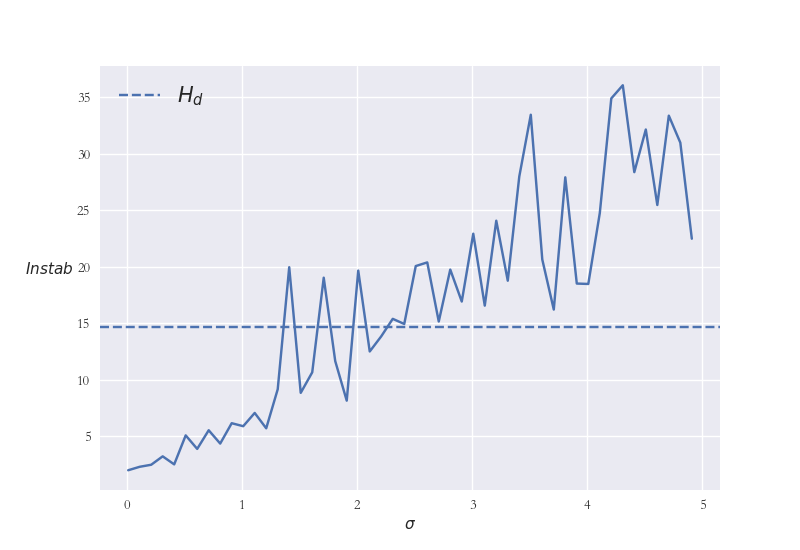
\includegraphics[width=0.9\linewidth]{高钾类玻璃稳定性分析.png}
		\caption{高钾类玻璃稳定性分析}
		\label{fig:高钾类玻璃稳定性分析}
		\end{subfigure}
		\caption{高钾类玻璃聚类分析结果和稳定性分析}
\end{figure}

\begin{figure}[H]
	\centering
	\begin{subfigure}[t]{0.48\linewidth}
		\centering
		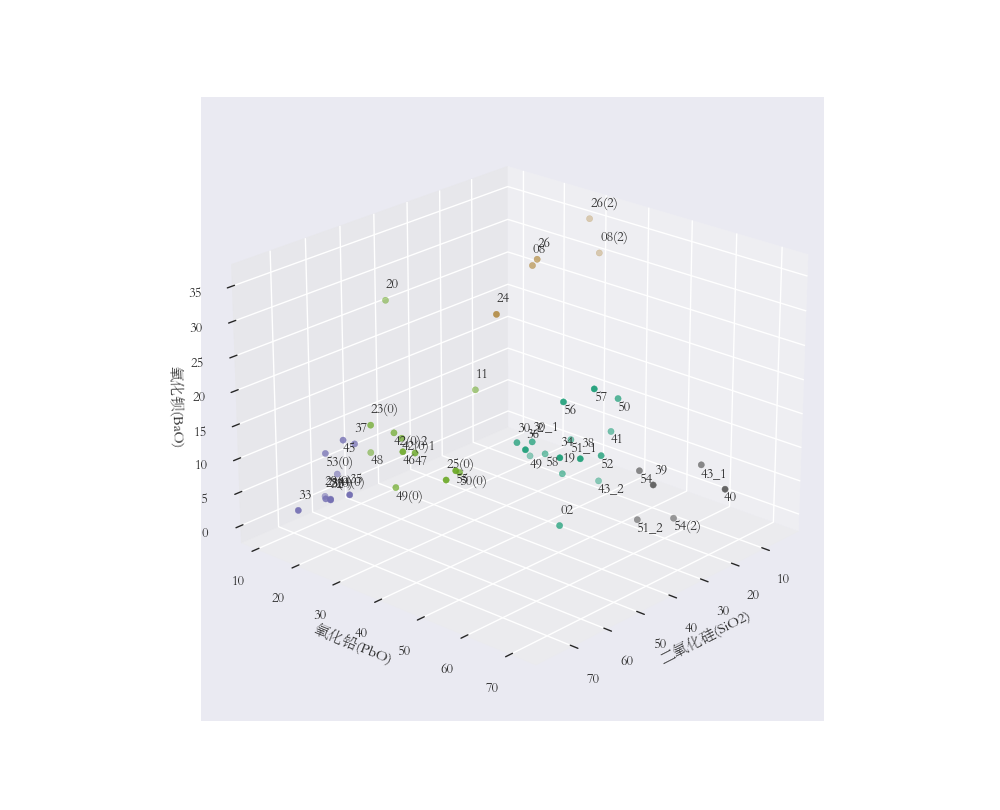
\includegraphics[width=0.9\linewidth]{铅钡类玻璃聚类分析结果.png}
		\caption{铅钡类玻璃聚类分析结果}
		\label{fig:铅钡类玻璃聚类分析结果}
		\end{subfigure}
		\begin{subfigure}[t]{0.48\linewidth}
		\centering
		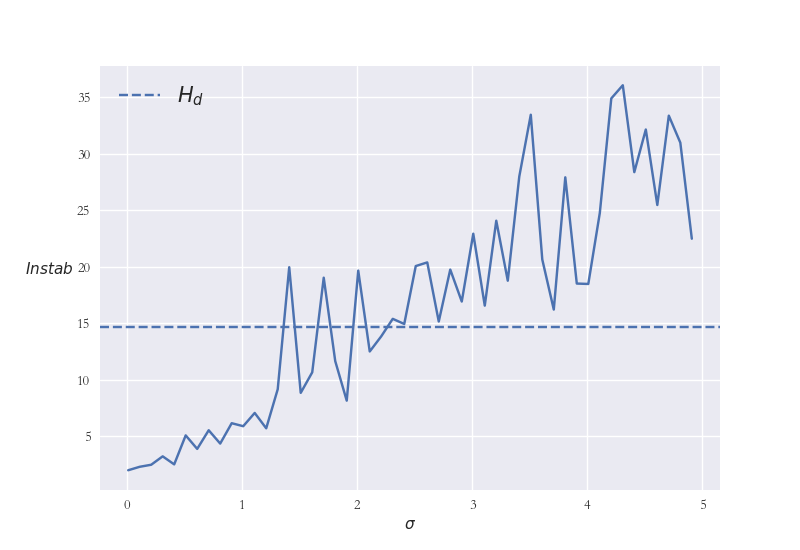
\includegraphics[width=0.9\linewidth]{高钾类玻璃稳定性分析.png}
		\caption{铅钡类玻璃稳定性分析}
		\label{fig:铅钡类玻璃稳定性分析}
		\end{subfigure}
		\caption{铅钡类玻璃聚类分析结果和稳定性分析}
\end{figure}
	
	得到聚类划分结果如图\ref{fig:高钾类玻璃聚类分析结果}和\ref{fig:铅钡类玻璃聚类分析结果}。为了简化图形标注,对铅钡样本聚类中文物采样点标注进行简写(例如:将30号样本部位1,2分别记为“30\_1,30\_2",将53号样本未风化点记为$53(0)$,将54号样本严重风化点记为54(2))。
	
	由聚类结果,$R_3$空间中铅钡玻璃样本点分为5个点集,用不同颜色标注,记为$C_i$ $(i=1,2,\cdots,5)$,将这5个不同聚类作为铅钡玻璃的亚类。同理,高钾玻璃样本点分为$R_2$中的3个点集,记为$D_i$ $(i=1,2,3)$,将这3个不同聚类作为高钾玻璃的亚类。
        划分结果如表\ref{tab:高钾类玻璃聚类结果}和\ref{tab:铅钡类玻璃聚类结果}所示,只展示了部分数据,全部数据见附录(******)
        
        % Table generated by Excel2LaTeX from sheet 'Sheet1'
\begin{table}[H]
	\centering
	\caption{高钾类玻璃聚类结果}
	  \resizebox{\textwidth}{!}{
		\begin{tabular}{ccccccccccccccccccc}
			\toprule
			\textbf{文物采样点} & 01    & 03部位1 & 03部位2 & 04    & 05    & 06部位1 & 06部位2 & 07    & 09    & 10    & 12    & 13    & 14    & 16    & 18    & 21    & 22    & 27 \\
			\midrule
			\textbf{类别} & 1     & 0     & 1     & 1     & 1     & 1     & 1     & 2     & 2     & 2     & 2     & 1     & 1     & 1     & 0     & 0     & 2     & 2 \\
			\bottomrule
			\end{tabular}%
	  }
	\label{tab:高钾类玻璃聚类结果}%
  \end{table}%
  
  % Table generated by Excel2LaTeX from sheet 'Sheet1'
\begin{table}[H]
	\centering
	\caption{铅钡类玻璃聚类结果}
	  \resizebox{\textwidth}{!}{
		\begin{tabular}{cccccccccccccccccc}
			\toprule
			\textbf{文物采样点} & 02    & 08    & 08(2) & 11    & 19    & 20    & 23(0) & 24    & 25(0) & 26    & 26(2) & 28(0) & 29(0) & 30\_1 & 30\_2 & 31    & 32 \\
			\midrule
			\textbf{类别} & 2     & 1     & 1     & 0     & 2     & 0     & 0     & 1     & 0     & 1     & 1     & 3     & 3     & 2     & 2     & 3     & 3 \\
			\midrule
			\textbf{文物采样点} & 33    & 34    & 35    & 36    & 37    & 38    & 39    & 40    & 41    & 42(0)1 & 42(0)2 & 43\_1 & 43\_2 & 44(0) & 45    & 46    & 47 \\
			\midrule
			\textbf{类别} & 3     & 2     & 3     & 2     & 3     & 2     & 4     & 4     & 2     & 0     & 0     & 4     & 2     & 3     & 3     & 0     & 0 \\
			\midrule
			\textbf{文物采样点} & 48    & 49    & 49(0) & 50    & 50(0) & 51\_1 & 51\_2 & 52    & 53(0) & 54    & 54(2) & 55    & 56    & 57    & 58    &       &  \\
			\midrule
			\textbf{类别} & 0     & 2     & 0     & 2     & 0     & 2     & 4     & 2     & 3     & 4     & 4     & 0     & 2     & 2     & 2     &       &  \\
			\bottomrule
			\end{tabular}%
	  }
	\label{tab:铅钡类玻璃聚类结果}%
  \end{table}%
	
	\subsection{合理性与敏感性检验}

	\subsubsection{合理性检验}
            
        \subsubsection{敏感性检验}
	对于传统的敏感性检验方法,是在原有模型基础上仅对测试样本加入噪声判断其所属分类是否变动,以此考量模型的稳健性,但考虑到传统方法在选择测试样本上的局限性,本文在论文(*****)提出的检验模型敏感性方法的基础上,对检验模型敏感性进行了进一步的创新。对所有测试数据加入高斯分布的噪声,重新进行聚类并比较其结果是否发生变化。基于所有测试数据的敏感性检验相比于单独抽取数据的传统敏感性检验,避免了抽样的随机性,获得了更全面的评价。
	

	首先在所有样本数据上均加入不同程度的Gauss噪声$g_k$($g_k\sim N(\mu ,\sigma_k^2 ),\sigma_k\in(0.01,5))$, $(k=1,2,\cdots,n)$,得到n组样本$\{X_1,X_2,\cdots,X_n\}$。
	
	具体算法原理如下:
	
	\begin{algorithm}[H]
	\caption{生成噪声数据集}
	\label{alg:生成噪声数据集}
	\begin{algorithmic}[1]
		\Require $X$
		\Ensure $X_1,X_2,\cdots,X_n$
		\State Initialization: i${\leftarrow}$1,${X_i=X,(i \in [1,n])}$
		\For{each ${\sigma \in (0.01,5)}$}
			\For{each ${X_i[i][j]}$  in ${X_i}$}
			\State ${X_i[i][j]}$+= random\_noise\quad //random\_noise $\sim N(0,\sigma^2)$
			\EndFor
		\EndFor
	\end{algorithmic}
\end{algorithm}

	其次对得到的$n$组新样本数据进行KMeans聚类分析,得到$n$组新的聚类分析结果。不妨记原数据样本为$X$,聚类后得到的点集集合记为$C$;对于新得到的$n$组样本$X_1,X_2,\cdots,X_n$,将第$i$组样本聚类分析后得到的点集集合记为$C_i$ $(i=1,2,\cdots,n)$。
    
    若利用传统计算点集之间最近的点的距离衡量两点集之间的差别,则在点集间普遍存在交错时,这一衡量便失去意义;且对于凸包形状不规则的点集,在利用传统质心距离衡量的过程中也会丧失点集分布的形状等信息,因此我们需要采用一种能保留更多信息度的距离。

    参考文献(****),我们采用了Hausdorff距离作为评价两点集是否接近的指标,这样既能避免点集普遍交错的问题,又能充分考虑点集的形状。
    
	定义
	\begin{equation}
	    \mr{Hd}(S,S_i')=\max_{a\in S}\left\{\min_{b\in S_i'}\{d(a,b)\}\right\}.
	\end{equation}
	Hd刻画了集合C中任意点到$S_i'$中最近点距离的最大值,可以作为衡量集合S,$S_i'$距离、偏移量或重合度的重要指标\cite{Huang2019}。
	
	不妨设聚类C由t个集合$S_k$构成,即$C=\bigcup_{k=1}^tS_k$。绘制随着噪声方差$\sigma$由0.01到5递增的新聚类$C_i$相对原聚类C的累计偏移值$Instab_{(C,C_i)}=\Sigma_{i\in [1,n]}dis_i$曲线,如图(*****)所示。
    在$\sigma\in[0.01,\sigma_0]$范围内,$(0.01<\sigma_0\leqslant 5)$,有
	\begin{equation}
	    \min_{i\neq j,S_i,S_j \in C}\mr{Hd}(S_i,S_j)\geqslant Instab_{(C,C_i)}.
	\end{equation}
	这就说明加入服从Gauss分布方差小于等于$\sigma_0$的噪声对样本点造成的偏移是有限的,对原有分类方式的改变不大。而在$\sigma>\sigma_0$ 范围下,噪声的干扰就会对样本点的分类方式造成显著影响。

    由图(****)可知,在$\sigma<1$的范围内,噪声的干扰对样本点的分类方式造成的改变不大。而现实中噪声干扰的$\sigma$通常在0.05一下,从而说明模型对于数据的随机误差波动时不敏感的,模型是稳健的。
    
    具体算法原理如下:
   
\begin{algorithm}[H]
	\caption{基于噪声扰动的分类模型敏感性分析}
	\label{基于噪声扰动的分类模型敏感性分析}
	\begin{algorithmic}[1]
		\Require $X,X_1,X_2,...,X_n$
		\Ensure	$Instab_{(C,C_1)},Instab_{(C,C_2)},...,Instab_{(C,C_n)}$
		\State Initialization: 对数据集$X,X_1,X_2,...,X_n$,用Kmeans进行聚类,得到聚类结果$C,C_1,C_2,...,C_n$. $C,C_i$都为点集的集合
		\Function{Hausdorff\_distance}{$S_1,S_2$}
		\Statex \quad //$S_1$,$S_2$为两个点集,Hausdorff\_distance函数为计算两个点集的距离
		\For{each $a\in S_1$}
		\Statex \qquad//对点集$S_1$中的每个点,找到点集$S_2$中欧氏距离距其最近的点$b$
		\State $dis_a \leftarrow \min_{b\in S_2}(\norm{a-b}_2)$
		\EndFor
		\qquad //找到两个集合所有相聚最距最近的点的距离最大值
		\State $dis_{(S1,S2)}\leftarrow \max_{a\in S_1}(dis_a)$
		
		\Return $dis_{(S1,S2)}$
		\EndFunction
		\For{each ${C_i,i\in [1,n]}$}
		\Statex \quad //对于每个加入噪声干扰数据$X_i$的聚类结果$C_i$,求其与原数据$X$的聚类结果$C$的差异
		 \For{each $S_k\in C$}
		 \State $dis_{S_k} \leftarrow \min_{S_l\in C_i}$(Hausdorff\_distance$ (S_k,S_l))$
		 \EndFor
		 \State $Instab_{(C,C_i)}\leftarrow \Sigma_{S_k\in C}(dis_{S_k})$
		\EndFor
	\end{algorithmic}
\end{algorithm}
	
	\section{问题三:}
	可根据题意依次对未分类样品进行类型划分与亚类细分,再分析分类结果的敏感性。首先将样品化学成分含量数据代入问题二中建立的SVM支撑向量机分类模型,再按玻璃类型代入对应的KMeans聚类分析模型,最后在样本数据加入不同程度的Gauss噪声,参照原始分类结果得出保持模型分类正确的噪声区间,证明模型稳健性。
	\subsection{类型与亚类归属}
	为通过化学成分分析鉴别文物类型,首先考虑将未分类样本点根据玻璃类型分为高钾玻璃和铅钡玻璃两大类。在问题二第一部分中我们建立SVM支撑向量机分类模型,求出了可以将不同类型玻璃样本完全分隔的最优支撑超平面,现将未分类样本点各项化学成分数据代入模型,即可通过判断样本点与超平面相对位置得到分类结果。
	求得的初步分类结果为:
	
	A1、A6、A7属于高钾玻璃,A2、A3、A4、A5、A8属于铅钡玻璃。

	其次为实现高钾和铅钡样本按亚类的细分,考虑利用问题二第二部分中建立的KMeans聚类分析模型,通过将样本点归在距离最近的聚类,实现对样本点所属亚类的判断。
		求得的细分结果为:	A1$\in$D2,A6、A7$\in$D0;A4、A8$\in$C4,A5$\in$C1
		
		
其中$C_i(i=1,2,\cdots,5)$为铅钡玻璃的聚类划分,$D_i(i=1,2,3)$为高钾玻璃的聚类划分。
	\subsection{敏感性分析}
	首先对判断玻璃类型的SVM支撑向量机分类模型进行敏感性分析,结合“采样检测可能导致的偏差通常呈均值为0的正态分布”这一生活实际,考虑在未分类样本中加上不同程度的Gauss噪声$t_k$($t_k\sim N(0 ,\sigma_k^2 ),\sigma_k\in(0.01,10),k=(1,2,\cdots,n)$,将得到的n组新数据代入已有的SVM支撑向量机分类模型。根据之前的判断结果,定义正确率为“加入噪声后样品点类型判断结果与原样品点类型相同的数目:原未分类样品总数”,绘制随$\sigma_k$在(0.01,10)间增大的判断正确率曲线如图(***)
	
	发现当$\sigma_k\in(0.01,4.5)$时,类型划分模型保持100\%正确率,说明SVM支撑向量机分类模型是稳健的。
	
	其次对判断高钾、铅钡玻璃所属亚类的KMeans聚类分析模型进行敏感性分析,出于相同考量,在高钾、铅钡玻璃样品数据上分别加上不同程度的Gauss噪声$r_k$($r_k\sim N(0 ,\sigma_k^2 ),\sigma_k\in(0.01,5),k=(1,2,\cdots,m)$,将得到的2m组新数据代入已有的KMeans聚类分析模型。同样绘制出随噪声方差在(0.01,5)之间逐步递增的判断正确率曲线如图(***)
	
	发现当$\sigma_k\in(0.01,1.5)$时,高钾玻璃、铅钡玻璃亚类划分模型均保持100\%正确率,说明的KMeans聚类分析模型是稳健的。
	\section{问题四:}
	为了分析不同类别文物之间化学成分的关联关系,以及关联关系的差异性,考虑到文物的类别如颜色、纹饰可能是多分类定类变量,因此采用方差分析法做出判断,再结合不同种类样品的化学成分含量平均值、标准差等基本信息和SVM支持向量机玻璃类型分划模型,综合文献得出关联及差异。
	\subsection{方差分析模型分类衡量成分差异}
	可将玻璃文物样品按玻璃类型、颜色、纹饰进行分类,下面分别考量不同种类玻璃文物样品间化学成分差异。不妨以颜色为例,首先根据文物表面的颜色对文物进行分类,由于附件表单2中文物一共呈现8种颜色,分别是黑色、蓝绿色、绿色、浅蓝色、浅绿色、深蓝色、深绿色、紫色,不妨对这几种颜色编上标号,记黑:1,蓝绿:2,绿:3,浅蓝:4,浅绿:5,深蓝:6,深绿:7,紫:8以便统计。考虑到附件表单1中部分文物并没有颜色数据,则将这些文物样本数据从附件2和附件1中剔除,实现数据的预处理。
	
	\textbf{\emph{Step 1.}}方差分析相关变量
	
	设文物的颜色种类为$D$,其中每种颜色划分种类为$D_1,\cdots,D_{8}$,对于一种固定的化学成分,令在种类$D_j(j=1,2,\cdots,8)$下的数据(也就是这一种类的文物的这个化学成分含量)的数量为$n_j$,再令$E_{ij}$为第$i$个种类的第$i$文物的该化学成分含量,那么得到下表:
	% Table generated by Excel2LaTeX from sheet 'Sheet1'
\begin{table}[H]
  \centering
  \caption{方差分析数据表}
  \renewcommand{\arraystretch}{1.5}
    \begin{tabularx}{\textwidth}{C|C|C|C|C}
    \hline
          &   $D_1$    &     $D_2$  &   $\cdots$    & $D_8$ \\
    \hline
    \multicolumn{1}{c|}{\multirow{4}[0]{*}{对应化学成分}} &   $E_{11}$    &   $E_{12}$   &  $\cdots$  & $E_{18}$ \\
    \cline{2-5}
     &   $E_{21}$    &  $E_{22}$     &   $\cdots$    & $E_{28}$ \\
     \cline{2-5}
          &   $\vdots$    &    $\vdots$   &       & $\vdots$ \\
          \cline{2-5}
          &   $E_{n_11}$    &   $E_{n_22}$    &    $\cdots$   & $E_{n_88}$ \\
          \hline
    样本总和  &    $T_{1}$   &  $T_2$     &    $\cdots$   & $T_8$ \\
    \hline
    样本均值  &   $\bar{E}_1$    &  $\bar{E}_2$     &   $\cdots$    & $\bar{E}_8$ \\
    \hline
    总体均值  &    $\mu_1$   &   $\mu_2$    &   $\cdots$    & $\mu_8$ \\
    \hline
    \end{tabularx}%
  \label{tab:addlabel}%
\end{table}%
    其中,令
    \begin{gather}
        n=n_1+\cdots+n_8\textbf{,}\\
        \bar{E_j}=\sum_{l=1}^8\sum_{i=1}^{n_j}E_{il}=n\bar{E}\text{。}
    \end{gather}
    
    \textbf{\emph{Step 2. }}因素水平
    
    \begin{enumerate}
        \item 颜色种类为$D_j$的样品化学含量水平$E_{1j},\cdots,E_{nj}$服从正态分布$N(\mu_j,\sigma^2)$,容量为$n_j$,其中$\mu_j,\sigma$未知。
        \item 在不同的样品中抽取的检测样本化学成分含量相互独立。
    \end{enumerate}
    
    \textbf{\emph{Step 3.}} 命题假设 
    检验不同种类玻璃样本化学成分含量均值。
    
    提出原假设为$H_0$.
    \begin{equation}
        H_0:\mu_1=\mu_2=\cdots=\mu_8\text{。}
    \end{equation}
    备择假设为$H_1$.
    \begin{equation}
        H_1:\mu_1,\mu_2,\cdots,\mu_8\text{不全相等。}
    \end{equation}
    
    \textbf{\emph{Step 4. }}模型构建及求解
    
    令
    \begin{gather}
        S_T=\sum_{k=1}^8\sum_{i=1}^{n_j}(E_{ik}-\bar{E})^2\text{,}\\
        S_E=\sum_{k=1}^8\sum_{i=1}^{n_j}(E_{ik}-\bar{E}_k)^2\text{,}\\
        S_A=S_T-S_E\text{。}
    \end{gather}
    
    若$H_0$为真,那么检验统计量满足
    \begin{equation}
        F=\frac{(n-8)S_A}{7S_E}\sim F(s-1,n-s)\text{,}
    \end{equation}
    对于给定的显著性水平$\alpha$,得到临界值$F_\alpha$,满足
    \begin{equation}
        P\left\{\frac{(n-8)S_A}{7S_E}>F_\alpha\right\}=\alpha\text{。}
    \end{equation}
    
     \subsection{结果分析}
    通常情况下,取临界值$F_\alpha$=0.01,将检验统计量与$F_\alpha$进行比较,得到结果如图(***)(这里仅截取所有显著性水平小于0.01的化学成分,详见附录**):

% Table generated by Excel2LaTeX from sheet 'Sheet4'
\begin{table}[H]
  \centering\small
  \caption{颜色分类的方差分析结果}
    \begin{tabularx}{\textwidth}{CCCCCC}
    \toprule
    \multicolumn{2}{C}{} & \multicolumn{1}{C}{平方和} & \multicolumn{1}{C}{自由度} & \multicolumn{1}{C}{均方} & \multicolumn{1}{r}{显著性} \\
    \midrule
    \multicolumn{1}{l}{\multirow{2}[4]{*}{二氧化硅(SiO2)}} & 组间    & 13598.4 & 6     & 2266.4 & \multicolumn{1}{r}{0.000} \\
\cmidrule{2-6}          & 组内    & 23438.3 & 56    & 418.541 &  \\
    \midrule
    \multicolumn{1}{l}{\multirow{2}[4]{*}{氧化铜(CuO)}} & 组间    & 137.403 & 6     & 22.901 & \multicolumn{1}{r}{0.000} \\
\cmidrule{2-6}          & 组内    & 192.853 & 56    & 3.444 &  \\
    \midrule
    \multicolumn{1}{l}{\multirow{2}[4]{*}{氧化铅(PbO)}} & 组间    & 6628.03 & 6     & 1104.67 & \multicolumn{1}{r}{0.005} \\
\cmidrule{2-6}          & 组内    & 17583.2 & 56    & 313.985 &  \\
    \midrule
    \multicolumn{1}{l}{\multirow{2}[4]{*}{氧化钡(BaO)}} & 组间    & 2482.82 & 6     & 413.804 & \multicolumn{1}{r}{0.000} \\
\cmidrule{2-6}          & 组内    & 2435.25 & 56    & 43.487 &  \\
    \midrule
    \multicolumn{1}{l}{\multirow{2}[4]{*}{氧化锶(SrO)}} & 组间    & 1.655 & 6     & 0.276 & \multicolumn{1}{r}{0.000} \\
\cmidrule{2-6}          & 组内    & 3.146 & 56    & 0.056 &  \\
    \midrule
    \multicolumn{1}{l}{\multirow{2}[4]{*}{氧化锡(SnO2)}} & 组间    & 3.357 & 6     & 0.560 & \multicolumn{1}{r}{0.000} \\
\cmidrule{2-6}          & 组内    & 2.940 & 56    & 0.052 &  \\
    \midrule
    \multicolumn{1}{l}{\multirow{2}[4]{*}{二氧化硫(SO2)}} & 组间    & 189.447 & 6     & 31.575 & \multicolumn{1}{r}{0.000} \\
\cmidrule{2-6}          & 组内    & 297.716 & 56    & 5.316 &  \\
    \bottomrule
    \end{tabularx}%
  \label{tab:addlabel}%
\end{table}%



   
    图中表明,$\mr{SiO_2}$等化学元素含量对应的显著性水平小于0.01,说明拒绝原假设“不同种类玻璃文物化学元素含量相等”,这表明在不同颜色的玻璃文物中,这些元素的含量差异巨大。
    
    可以推测:这些化学成分含量差异是导致文物呈现不同颜色的原因,结合对数据平均值、标准差、均方等基本数学信息的统计(详见附录**),还可以得出更为具体的信息,如:SrO组内标准差小,这表明相同颜色玻璃文物的SrO含量差异较小。
    
% Table generated by Excel2LaTeX from sheet 'Sheet2'
\begin{table}[H]
  \centering\small
  \caption{纹饰分类的方差分析结果}
    \begin{tabularx}{\textwidth}{CCCCCC}
    \toprule
    \multicolumn{2}{C}{} & \multicolumn{1}{C}{平方和} & \multicolumn{1}{C}{自由度} & \multicolumn{1}{C}{均方} & \multicolumn{1}{r}{显著性} \\
    \midrule
    \multicolumn{1}{l}{\multirow{2}[4]{*}{氧化钠(Na2O)}} & 组间    & 11.5871 & 2     & 5.79357 & \multicolumn{1}{r}{0.13341} \\
\cmidrule{2-6}          & 组内    & 178.34 & 64    & 2.78656 &  \\
    \midrule
    \multicolumn{1}{l}{\multirow{2}[4]{*}{氧化钾(K2O)}} & 组间    & 23.9806 & 2     & 11.9903 & \multicolumn{1}{r}{0.47164} \\
\cmidrule{2-6}          & 组内    & 1009.14 & 64    & 15.7678 &  \\
    \midrule
    \multicolumn{1}{l}{\multirow{2}[4]{*}{氧化钙(CaO)}} & 组间    & 20.4238 & 2     & 10.2119 & \multicolumn{1}{r}{0.16911} \\
\cmidrule{2-6}          & 组内    & 357.632 & 64    & 5.58801 &  \\
    \midrule
    \multicolumn{1}{l}{\multirow{2}[4]{*}{氧化铁(Fe2O3)}} & 组间    & 8.17821 & 2     & 4.0891 & \multicolumn{1}{r}{0.05688} \\
\cmidrule{2-6}          & 组内    & 87.261 & 64    & 1.36345 &  \\
    \midrule
    \multicolumn{1}{l}{\multirow{2}[4]{*}{氧化铜(CuO)}} & 组间    & 11.5614 & 2     & 5.78071 & \multicolumn{1}{r}{0.33278} \\
\cmidrule{2-6}          & 组内    & 330.505 & 64    & 5.16414 &  \\
    \midrule
    \multicolumn{1}{l}{\multirow{2}[4]{*}{五氧化二磷(P2O5)}} & 组间    & 61.287 & 2     & 30.6435 & \multicolumn{1}{r}{0.10499} \\
\cmidrule{2-6}          & 组内    & 839.853 & 64    & 13.1227 &  \\
    \midrule
    \multicolumn{1}{l}{\multirow{2}[4]{*}{氧化锡(SnO2)}} & 组间    & 0.41855 & 2     & 0.20928 & \multicolumn{1}{r}{0.17411} \\
\cmidrule{2-6}          & 组内    & 7.45464 & 64    & 0.11648 &  \\
    \midrule
    \multicolumn{1}{l}{\multirow{2}[4]{*}{二氧化硫(SO2)}} & 组间    & 23.4408 & 2     & 11.7204 & \multicolumn{1}{r}{0.20746} \\
\cmidrule{2-6}          & 组内    & 465.295 & 64    & 7.27024 &  \\
    \bottomrule
    \end{tabularx}%
  \label{tab:addlabel}%
\end{table}%





    
    同理,对不同纹饰玻璃样品化学成分含量数据进行方差分析,结果如图(***),可以发现符合方差齐性的化学成分所对应的显著性均大于0.05,说明不同纹饰玻璃文物间化学成分含量无明显差异。
    
    对于不同类型的玻璃样品,在6.1中已通过SVM分类机模型进行划分,记
    $$H(x)=(\bm{\omega} \cdot \bm{x})+b$$
  其中$\bm{x}\in \mathbb{R}^{14}$
    $\bm{\omega} =(-0.02956241,0.00551535,-0.05283312,-0.01644926,-0.00040758,0.03743216,\\-0.02505811,-0.01378527,0.10249466,0.01348478,-0.02241906,0.00158788,0,0)$
  
  $b=1.1452272$
  
  对铅钡玻璃化学成分含量样本点$x_0$,有$H(x_0)$>0;
  
  对高钾玻璃化学成分含量样本点$x_1$,有$H(x_0)$<0。
  
  $\bm{\omega}$中第3、7、11项指标均为负,且绝对值较大,说明这些指标对应的化学元素$\mr{K_2O}$、$\mr{Fe_2O_3}$、$\mr{P_2O_5}$含量越高$H(x)$越小,样本点越容易出现在超平面下部,玻璃类型越可能为高钾玻璃。
  
  $\bm{\omega}$中第6、9、10项指标均为正,且绝对值较大,说明这些指标对应的化学元素$\mr{Al_2O_3}$、PbO、BaO含量越高$H(x)$越大,样本点越容易出现在超平面上部,玻璃类型越可能为高钾玻璃。
	\section{模型的评价与推广}
	\subsection{模型的优缺点}
	1)第一问运用变量间相互关系的卡方检验和独立样本的t检验,对于关系和统计规律的刻画比较客观和深刻。
	
	2)第二问使用SVM分类机,可以基于小样本进行学习和分类,大大简化了分类和判断的过程。同时,第二问使用了KMeans聚类分析来划分亚类,KMeans方法分割与数据的数量大致呈线性关系,时间复杂度较低,分类算法比较高效,结果比较准确。
	
	3)第四问用方差分析的方法,检验了以颜色、纹饰为分类依据时处理多个类别间每种化学成分的关联以及差异,具有完整性与直观性。
	
	4)对风化前玻璃化学成分含量的预测只是得到各个化学成分的范围,未能给出具体的数值,而且Kmeans的结果和运行时间与初始质心的选取有一定影响,对于不同的质心选取,结果和效率可能会存在差异。
	
	\subsection{模型的推广}
	第二问中运用SVM根据化学成分含量来对古代玻璃类型进行判断并用KMeans进行更细致的亚类划分,可以应用于考古学中对出土的未知类型但已知各个化学成分含量的古代玻璃文物进行定量分析的研究,模型对玻璃的类型进行客观的判断和分类,克服了人工分类的不准确性和模糊性。
	%参考文献
	\bibliographystyle{gbt7714-numerical}
	\bibliography{ref}
	
	%附录
	\newpage
	\begin{appendices}
		\begin{flushleft}
		    \textbf{附录清单}
		\end{flushleft}
		\begin{enumerate}
		        \item 第一问
		        \begin{enumerate}
		            \item BD\_poly.m
                \item curve\_K.m
                \item curve\_Pd.m
                \item prediction\_K.py
                \item prediction\_Pd.py
                \item 卡方检验.sav
                \item 高钾t检验.sav
                \item 铅钡t检验.sav
                \item 卡方检验-输出.spv
                \item 高钾t检验-输出.spv
                \item 铅钡t检验-输出.spv
                \item 频数统计表.xlsx
                \item 历史预测数据输入.xlsx
                \item 高钾类玻璃包络线拟合结果.xlsx
                \item 高钾类玻璃未风化化学成分预测结果.xlsx
                \item 铅钡类玻璃包络线拟合结果.xlsx
                \item 铅钡类玻璃未风化化学成分预测结果.xlsx
                \item 高钾类玻璃包络线拟合.png
                \item 铅钡类玻璃包络线拟合.png
		        \end{enumerate}
		        \item 第二问
		        \begin{enumerate}
                    \item SVM.pkl
                    \item ClusterK.pkl
                    \item ClusterPd.pkl
                    \item SVM.py
                    \item ClusterK.py
                    \item ClusterPd.py
                    \item ClusterK\_steady\_analy.py
                    \item ClusterPd\_steady\_analy.py
                    \item SVM输入.xlsx
                    \item Cluster输入.xlsx
                    \item 高钾类玻璃聚类结果.xlsx
                    \item 铅钡类玻璃聚类结果.xlsx
                    \item 高钾类SSE.png
                    \item 高钾类玻璃聚类分析结果.png
                    \item 高钾类玻璃稳定性分析.png
                    \item 铅钡类SSE.png
                    \item 铅钡类玻璃聚类分析结果.png
                    \item 铅钡类玻璃稳定性分析.png
		        \end{enumerate}
		        \item 第三问
		        \begin{enumerate}
                    \item SVM.pkl
                    \item ClusterK.pkl
                    \item ClusterPd.pkl
                    \item predict\_K\_Pd.py
                    \item predict\_K\_subgroup.py
                    \item predict\_Pd\_subgroup.py
                    \item sensitivity\_K\_Pd.py
                    \item 表单3.xlsx
                    \item 分类为高钾\_铅钡的稳定性.png
                    \item 子类稳定性.png
		        \end{enumerate}
		        \item 第四问
		        \begin{enumerate}
		            \item 方差分析纹饰.sav
                    \item 方差分析颜色.sav
                    \item 方差分析纹饰-输出.spv
                    \item 方差分析颜色-输出.spv
		        \end{enumerate}
		    \end{enumerate}
		    \section{MATLAB程序}
		    \subsection{第一问}
		    
	\end{appendices}
	
\end{document} 
